\begin{figure}[t]
\centering
\newcommand\antwidth{0.12}
\newcommand\humanoidwidth{0.16}
\subfloat[\texttt{Ant-length-mass}]{
\begin{tabular}{c}
\addvbuffer[0pt 0pt]{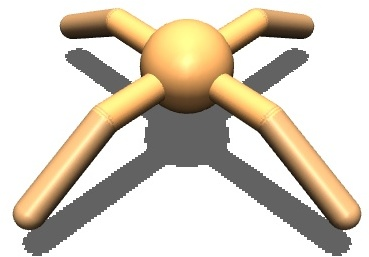
\includegraphics[width=\antwidth\textwidth, valign=m]{Figures/gym/ant_leg_length_mass_interp_0.00.jpg}} $\rightarrow$ \addvbuffer[0pt 0pt]{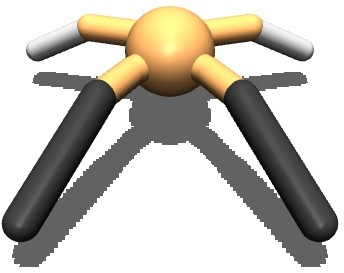
\includegraphics[width=\antwidth\textwidth,valign=m]{Figures/gym/ant_leg_length_mass_interp_1.00.jpg}}
\end{tabular} 
} 
\\
\vspace{-3ex}
\subfloat[\texttt{Humanoid-length-mass}]{
\begin{tabular}{c}
\addvbuffer[0pt 0pt]{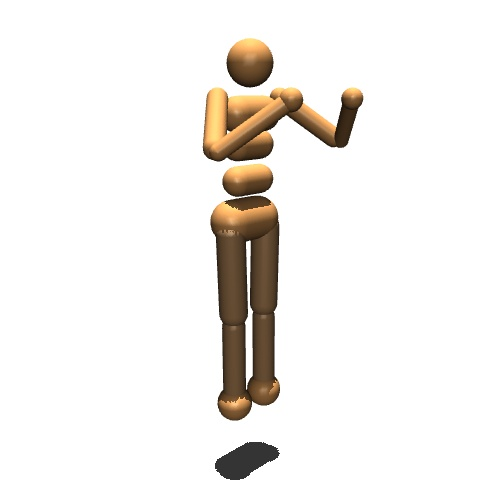
\includegraphics[height=\humanoidwidth\textwidth, valign=m]{Figures/gym/huamoid_leg_length_mass_interp_0.00.jpg}} $\rightarrow$ \addvbuffer[3pt 0pt]{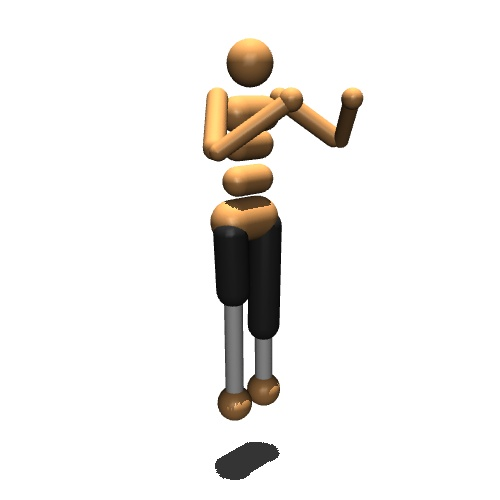
\includegraphics[height=\humanoidwidth\textwidth,valign=m]{Figures/gym/huamoid_leg_length_mass_interp_1.00.jpg}} 
\end{tabular} 
} 
\\
\vspace{-2ex}
\subfloat[\texttt{Ant-leg-emerge}]{
\begin{tabular}{c}
\addvbuffer[0pt 0pt]{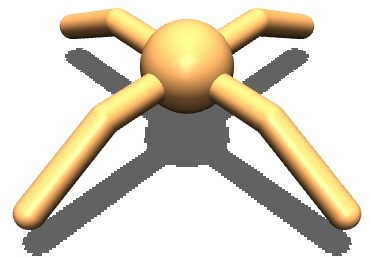
\includegraphics[width=\antwidth\textwidth, valign=m]{Figures/gym/ant_leg_emerge_interp_0.00.jpg}} $\rightarrow$ \addvbuffer[3pt 0pt]{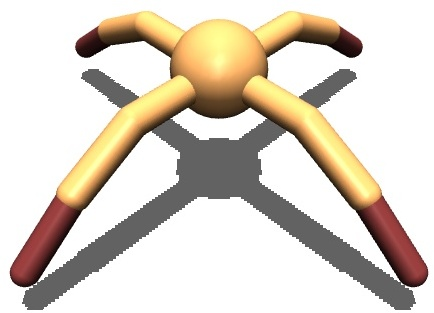
\includegraphics[width=\antwidth\textwidth,valign=m]{Figures/gym/ant_leg_emerge_interp_1.00.jpg}} \\
\end{tabular}
} 
\caption{Source-to-target robot evolution in the MuJoCo Gym environment used in experiments.
}
\end{figure}

